%%%%% this line is 80 chars wide, please don't make longer lines %%%%%%%%%%%%%%%
Let us speak now about the model of the peripheral auditory system from 
\cite{Model1, Model2, Model3}, used to run experiments in this project. 

We will not go into the details of the model, but we will speak more about the use of it. 
You can see in \autoref{fig:modelsch} the schematic of the model.


%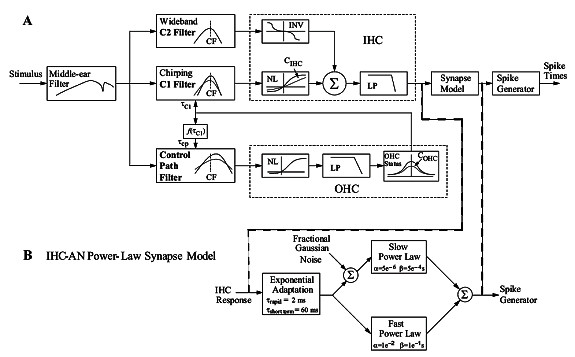
\includegraphics[width=0.45\textwidth]{images/www-bme-rochester-edu-schematicDiagram-level.jpg} %put in auditsys

From the user point of view, the model consists of two main functions 
that are called "catmodel\_IHC" and "catmodel\_Synapse". Their prototype is

\texttt{vihc = catmodel\_IHC(pin, CF, nrep, tdres, reptime, cohc, cihc);}

and

\texttt{[synout, psth] = catmodel\_Synapse(vihc, CF, nrep, tdres, fibertype, implnt);}

like specified in the "catmodel.m" file of the model. 
Let us go deeper into what each parameters and return value of these functions mean.

The first function, \texttt{catmodel\_IHC}, takes as parameters 
a stimulus vector (\texttt{pin}, in Pa), sampled at some sampling rate that corresponds 
to the bin size \texttt{tdres} (i.e. is the inverse of it), and 
the characteristic frequency (\texttt{CF}, in Hz) 
of the IHC and for which we want to know the potential 
(\texttt{vihc}, in Volt) when stimulated. 
This last thing (\texttt{vihc}) is what is returned by the function. 
\texttt{reptime} is the time for one repetition of the stimulus, 
and \texttt{nrep} is the number of repetions we want to be run. 
\texttt{cohc} and \texttt{cihc} represents the damages on respectively 
the outer hair cells and inner hair cells in the simulation.
\texttt{vihc} will contain the IHC potential for every repetition 
after the function has been run.

The second function, \texttt{catmodel\_Synapse}, 
takes the IHC potential returned by \texttt{catmodel\_IHC}, 
with the same sampling rate, so the same \texttt{tdres}, which is also here the bin size
of the PSTH returned by the function (\texttt{psth}). 
The PSTH will be computed according to the specified number of repetitions (\texttt{nrep}).
The synapse output of the IHC (\texttt{synout}) is also returned by the function.
The \texttt{fibertype} parameter is used to tell the model which nerve fiber type
we "test" with the stimulus, distinguished by their spontaneus rate (SR) : 
low, medium or high (low : $<$ 1 spike/s, medium : $<$ 18 spike/s, high: 20-50 spike/s, 
according to \cite{AuditoryNeuroscience}). %82
Finally, \texttt{implnt} is used to indicate the precision we want in the simulation 
for the power-law functions in the model.

As an example of what kind of result the model can give,
in \autoref{fig:g4tonestep} you can see some graphs that represents the steps of a 
simulation of a pure tone step stimulus.
A nerve fiber with high SR with a 1 kHz characteristic frequency 
was chosen.

%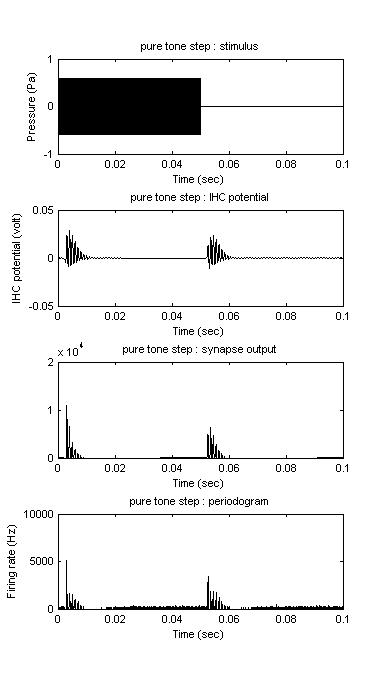
\includegraphics[width=0.45\textwidth]{images/g4-tonestep-column2.jpg}

\begin{figure}[h]
	\centering
	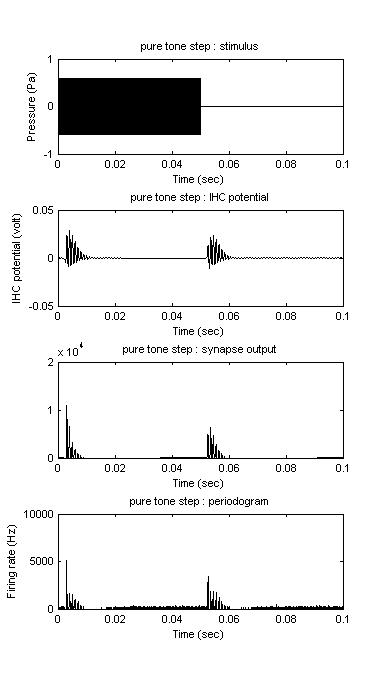
\includegraphics[width=0.45\textwidth]{images/g4-tonestep-column2.jpg}
	\caption{Example of model results (\cite{Model1})}
	\label{fig:g4tonestep}
\end{figure}


The first graph is a representation of one period of the stimulus, 
sampled at 100'000 Hz (so with bins of 0.01 ms size), at 84dB SPL.
What was given to the model as \texttt{pin} was this period of 100 ms repeated 800
times. The frequency of the pure tone is so high here (10 Hz) that we cannot see its sinusoid.
On the second graph, you can see the IHC potential from the first function
in response of the last period of the stimulus 
(with dependencies on the preceding periods included).
The third graph shows you a part of the synapse output given by \texttt{catmodel\_Synapse}, 
for the same period as for the potential of IHC.
The fourth graph represents the periodogram for the entire stimulus, 
computed with help of the PSTH given by the second function of the model.

For the project, the code of the model has been modified to put to zero 
the absolute refractory period (ARP) of nerve fibers. 
This transformation was done in the spike generator 
part of the model (see in \autoref{fig:modelsch} the last step on the right).
After that, the spike trains with and without this refractory period could be compared.

In \autoref{fig:psthcomp} you can see an example of a graph
where are drawn two periodograms, calculated from the PSTH given by the model 
(either modified or not), for another stimulus as before, a pure tone
which is not modulated.

%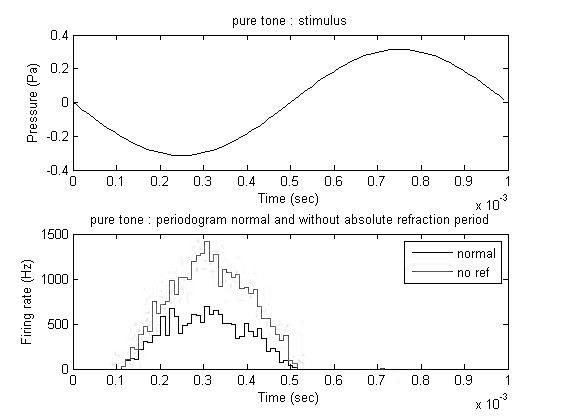
\includegraphics[width=0.45\textwidth]{images/stim-psth-puretone-bw2.jpg}

\begin{figure}[h]
	\centering
	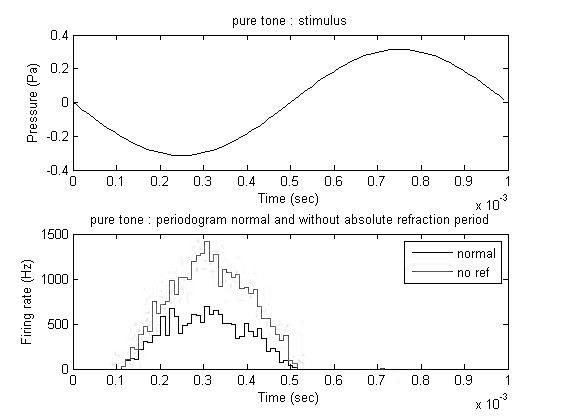
\includegraphics[width=0.5\textwidth]{images/stim-psth-puretone-bw2.jpg}
	\caption{Periodogram with and without refractory period for the stimulus of period above}
	\label{fig:psthcomp}
\end{figure} 

On the first graph, you can see one period of the stimulus, 
a 1 kHz pure tone, at 84dB SPL.
The second graphs shows you the periodogram with and without absolute refractory period.
We can see phase-locking for the two periodograms, so we see that the phase caracteristics 
of nerve seems not to change when the refractory period changes.
The simulation was done here with a medium SR nerve fiber, 
with 1 kHz characteristic frequency and 100 ms bin size.
We will see now the results of the project.

%\begin{lstlisting}[caption={},captionpos=b]{}
%\end{lstlisting}

%\texttt{tdres} 

 





